%%%%%%%%%%%%%%%%%%%%%%%%%%%%%%%%%%%%%%%%%%%%%%%%%%%%%%%%%%%%%%%%%%%%%%%%%%%%%%%%
%2345678901234567890123456789012345678901234567890123456789012345678901234567890
%        1         2         3         4         5         6         7         8

\documentclass[letterpaper, 10 pt, conference]{ieeeconf}  % Comment this line out
                                                          % if you need a4paper
%\documentclass[a4paper, 10pt, conference]{ieeeconf}      % Use this line for a4
                                                          % paper
\usepackage{graphicx}
\usepackage{amsmath}
\usepackage{graphicx}

\IEEEoverridecommandlockouts                              % This command is only
                                                          % needed if you want to
                                                          % use the \thanks command
\overrideIEEEmargins
% See the \addtolength command later in the file to balance the column lengths
% on the last page of the document

% The following packages can be found on http:\\www.ctan.org
%\usepackage{graphics} % for pdf, bitmapped graphics files
%\usepackage{epsfig} % for postscript graphics files
%\usepackage{mathptmx} % assumes new font selection scheme installed
%\usepackage{times} % assumes new font selection scheme installed
%\usepackage{amsmath} % assumes amsmath package installed
%\usepackage{amssymb}  % assumes amsmath package installed

\title{\LARGE \bf
Better Tools for Fault Diagnosis in Complex Systems\\
}

\author{Nathaniel Guy and Nick Reiter% <-this % stops a space
\thanks{Nathaniel Guy and Nick Reiter are both Masters students in the University of Washington Department of Computer Science and Engineering, and can be reached at {\tt\small natguy@cs.washington.edu} and {\tt\small nreiter@cs.washington.edu}, respectively.}%
}

\begin{document}

\maketitle
\thispagestyle{empty}
\pagestyle{empty}

%%%%%%%%%%%%%%%%%%%%%%%%%%%%%%%%%%%%%%%%%%%%%%%%%%%%%%%%%%%%%%%%%%%%%%%%%%%%%%%%
\begin{abstract}

Determining the root causes of problems for complex electromechanical systems is difficult. Systems can detect fault states quite reliably using simulated software models; however, even when a fault is detected, it can be difficult to determine the underlying reasons, and resolution method, for that fault. Some anticipated faults may be automatically recovered from, but others are more complex and require humans to understand their root causes before resolving them.

In this paper, we discuss the work that we've done to address these issues within a data visualization product. We discuss the major frontend components, as well as our highly modularized backend, which we developed in order to make a system that not only simplifies the telemetry monitoring and fault diagnosis tasks, but does it in a way that's extensible to a wide variety of systems.

\end{abstract}

%%%%%%%%%%%%%%%%%%%%%%%%%%%%%%%%%%%%%%%%%%%%%%%%%%%%%%%%%%%%%%%%%%%%%%%%%%%%%%%%
\section{INTRODUCTION}

The fault diagnosis process is very difficult, and can take weeks to months. It involves intense scrutiny of potentially thousands of data channels, and often the only comprehensive understanding of how these data channels relate to each other is encoded in human “tribal knowledge.” For this reason, a large amount of domain expertise is required to even begin this process.

Because diagnosing the root cause of system faults can take thousands of man-hours of expert time, any tools that can facilitate the navigation and organization of this task can potentially save a lot of money and time. However, visualizations designed for telemetry monitoring and fault diagnosis encounter the following major issues:

\begin{itemize}
  \item Displaying data from thousands of different channels isn't practical
  \item It is unclear how best to organize thousands of different interrelated channels to make interesting ones findable
  \item We would like to have automatic discovery and visualization of relationships between channels
  \item The tools ought to be able show many views of data in a coherent interface
\end{itemize}

Modern research has made some headway on these issues, and we have attempted to incorporate some of their findings within our project. Much of our organization and choice of components was influenced by personal experience with telemetry monitoring and analysis software used within the space industry, and the issues that we experienced first-hand when dealing with the problem of fault diagnosis across huge datasets.

%%%%%%%%%%%%%%%%%%%%%%%%%%%%%%%%%%%%%%%%%%%%%%%%%%%%%%%%%%%%%%%%%%%%%%%%%%%%%%%%
\section{RELATED WORK}

There is a rich body of literature related to telemetry visualization techniques and fault diagnosis. We borrowed insight and several visualization techniques from the literature. Cancro et al. developed useful techniques for packing large numbers of channels into a dense rectangular space \cite{Cancro}, and Yairi et al. demonstrated ways to show change correlation between data channels \cite{Yairi}, which were inspirations for our Global Correlation Matrix and Channel Correlation Vector. Simple fault detection methodology was adapted from Willsky \cite{Willsky}.

%%%%%%%%%%%%%%%%%%%%%%%%%%%%%%%%%%%%%%%%%%%%%%%%%%%%%%%%%%%%%%%%%%%%%%%%%%%%%%%%
\section{COMPONENT ARCHITECTURE}

We incorporated many different ideas from the fields of data visualization, and examined historical tools and theories for ideas. In this section, we give descriptions and justifications of components we implemented.

\subsection{Fault Monitoring Window}

Borrowing from traditional monitoring interfaces, this part of the visualization has a traditional live data display panel, including the current system time and values of specified telemetry channels. Which channels' values are shown is configurable.

This window also carries a description of any recent faults, along with details of the rules that originally caused them to trigger, and any other additional fault-related notes that system designers or operators have included for reference. This additional information, uncommon in traditional fault monitoring system, accelerates the fault diagnosis problem by immediately pointing towards possible root causes. Finally, an LED-shaped icon shows the current fault state, in order to quickly grab the attention of the operator. This section is designed to allow quick and easy viewing of critical and important information. See Figures~\ref{fig:monitor1} and \ref{fig:monitor2}.

\begin{figure}[h]
\centering
    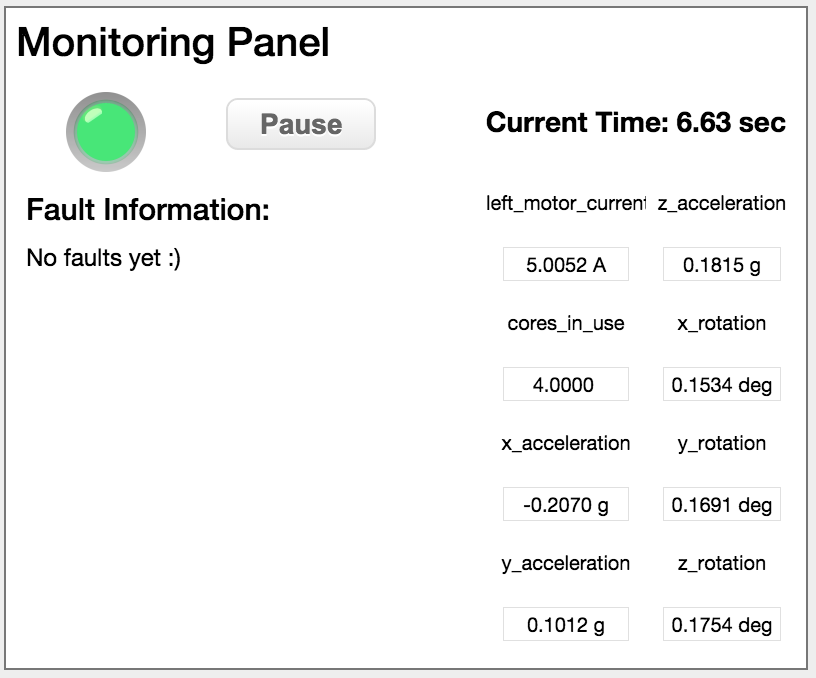
\includegraphics[width=0.6\columnwidth]{monitor12.png}
    \caption{An example of the default Fault Monitoring Window state.}
    \label{fig:monitor1}
\end{figure}

\begin{figure}[h]
\centering
    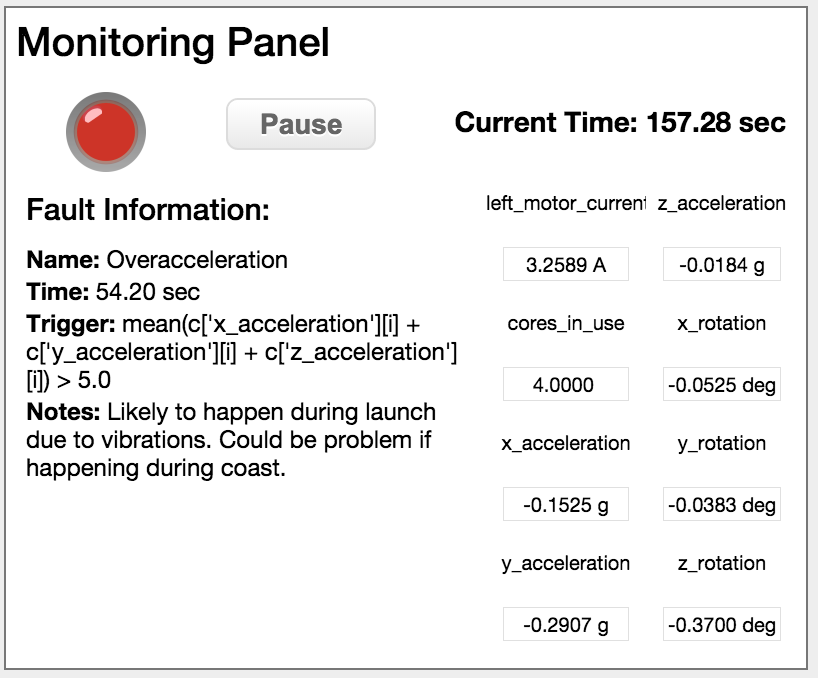
\includegraphics[width=0.6\columnwidth]{monitor22.png}
    \caption{An example of the faulted state of the Fault Monitoring Window.}
    \label{fig:monitor2}
\end{figure}

\subsection{Channel Hierarchy Window}

A degree-of-interest tree displays the hierarchy of all of the data channels. Major systems are broken into subsystems, which are then again broken into smaller subsystems, until the channels are reached at the leaf nodes. Clicking allows for expansion and navigation of the tree, and allows channel data to be selectively added to the Plotting Window. When a fault occurs, any related nodes on the tree are flagged, and those flags are propagated upwards to allow an operator to trace through the tree to find the channels affected by faults. Simple JSON configuration controls the organization, allowing for easy creation and customization for individual requirements. See Figure~\ref{fig:plots}.

\begin{figure}[h]
\centering
    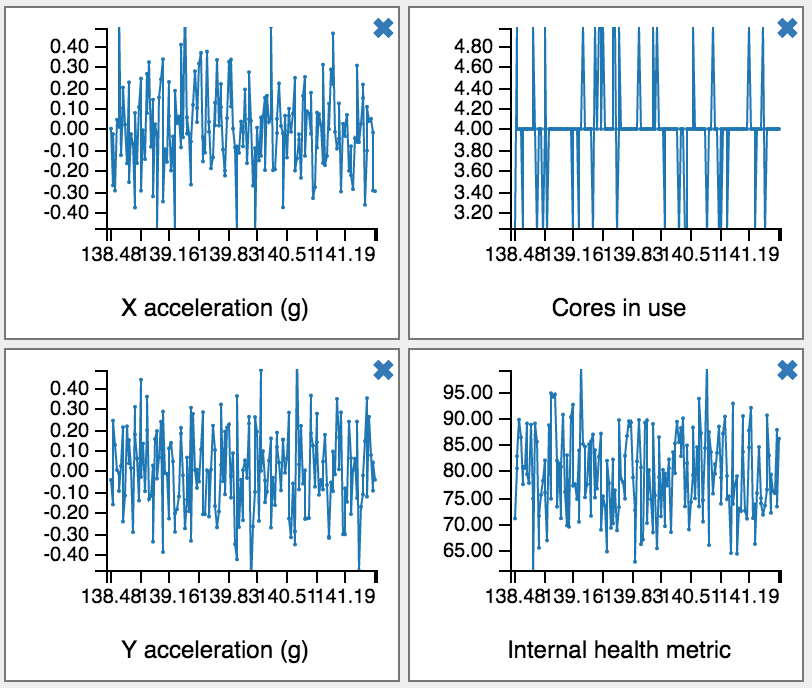
\includegraphics[width=\columnwidth]{plots2.png}
    \caption{Several examples of detail plots for various channels.}
    \label{fig:plots}
\end{figure}

\subsection{Plotting Window}

This component provides a set of configurable plots of live or time-relevant telemetry channel data. The plots update as new data comes in over the network. This component is tightly linked to the Channel Hierarchy Window, which provides an interface for adding new channels to be displayed. When a fault occurs, the channels determined to be most relevant to that fault are shown. Even in a fail-safe mode where no new telemetry is being received, the plot display allows a human operator to review data leading up to the fault. See Figure~\ref{fig:hierarchy}.

\begin{figure*}
\centering
    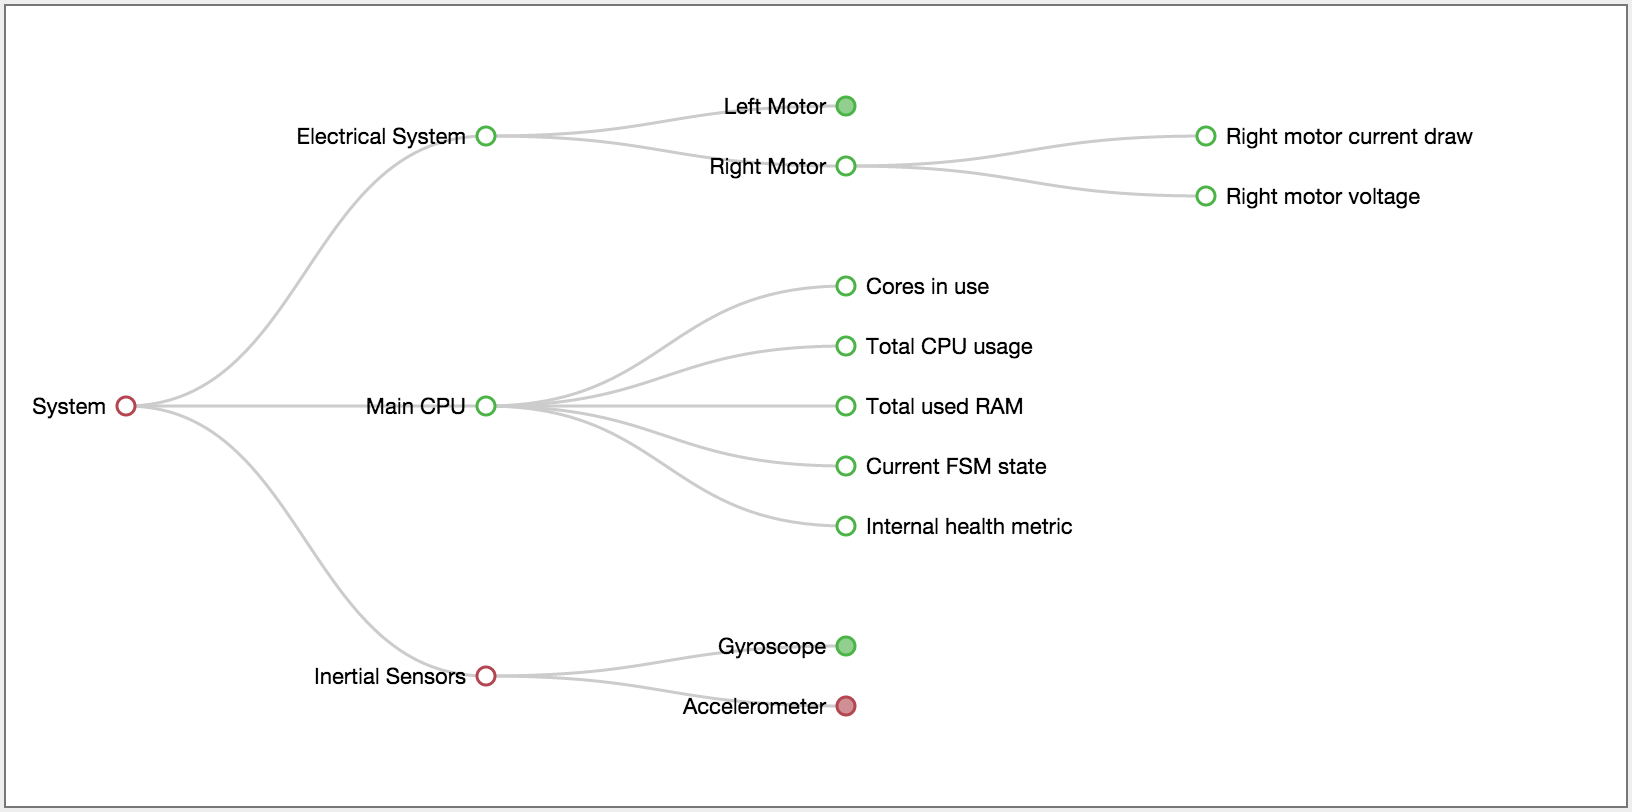
\includegraphics[width=\textwidth]{hierarchy2.png}
    \caption{The Channel Hierarchy Window expanded to show several subsystems, highlighting a fault in the Accelerometer subsystem.}
    \label{fig:hierarchy}
\end{figure*}

\subsection{Global Correlation Matrix}

This 2D matrix shows Pearson Correlation Coefficients across many different data channels, based on the most recent telemetry channel values. These cross-correlations are visualized using hue to show positive/negative correlation, and intensity to show the strength of that correlation. With this widget, an operator can see changing channel correlations, which may suggest possible interconnectedness or causation, based on more than physical or system connections. See Figure~\ref{fig:gcm}.

\begin{figure}[h]
\centering
    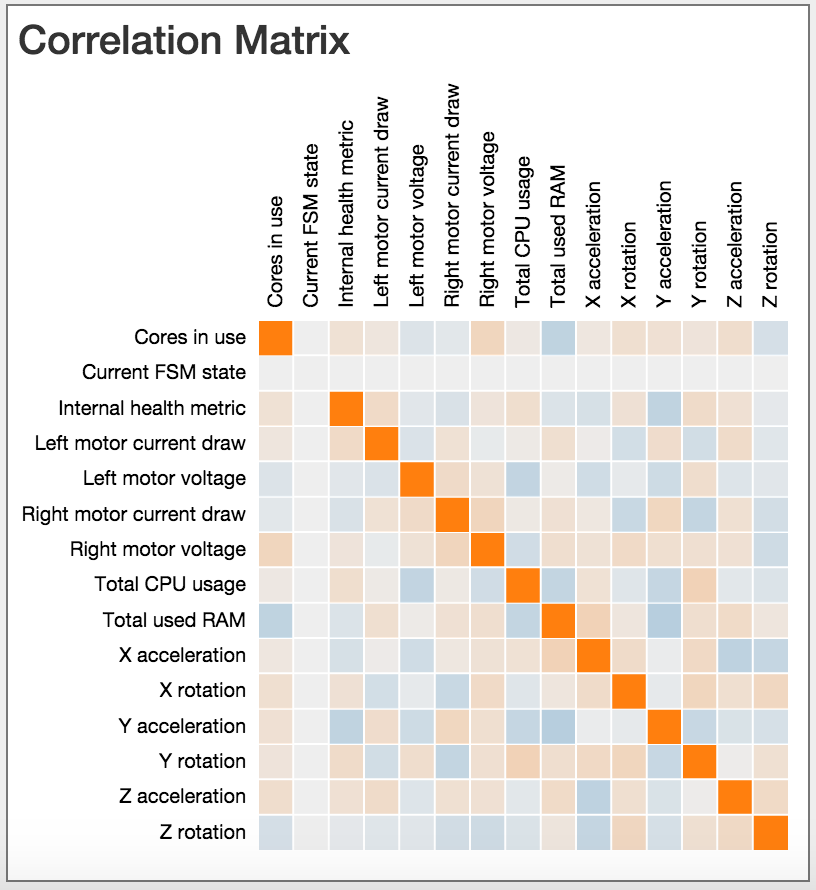
\includegraphics[width=\columnwidth]{gcm2.png}
    \caption{An example of the Correlation Matrix display.}
    \label{fig:gcm}
\end{figure}

\subsection{Channel Correlation Vector}

This component is similar to the Global Correlation Matrix, but shows channel correlations for a specific channel under review. Here, with the focus on an individual channel, we sort based on the magnitude of the correlation, and display the top related channels. The names of correlated channels are displayed for quick reference and faster lookup than the Global Correlation Matrix could provide.  See Figure~\ref{fig:cv}.

\begin{figure}[h]
\centering
    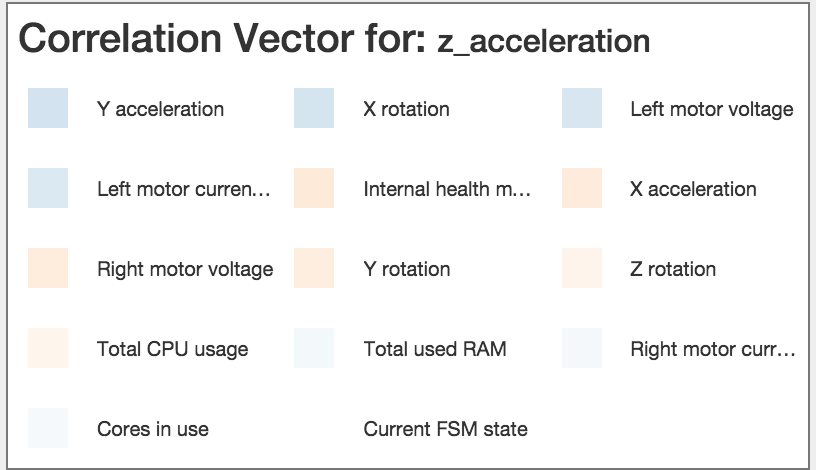
\includegraphics[width=\columnwidth]{cv2.png}
    \caption{An example of the Correlation Vector, focused on the Z Acceleration channel.}
    \label{fig:cv}
\end{figure}

\subsection{Additional Features}

We implemented a number of additional changes to the application that differentiate it from traditional telemetry monitoring interfaces and improve its applicability to a wide variety of systems and problems:

\subsubsection{JSON Configuration}

The application reads in component configuration from JSON files, including for the channel hierarchy, and the alarm system. This allows simple customization based on individual requirements. In particular, this provides a paradigm which makes modular development possible, where separate groups build up configuration for the components under their control. To generate the system config, these channel hierarchies can simply be collated, and the alarms collected. Additionally, the format is easily human-readable and editable.

\subsubsection{Automatic Fault Detection}

Organization using similar telemetry systems often have a set of fault detections rules, built up from experience and an understanding of the component engineering. The configuration mentioned above allows easy integration of these rules, both simple and complex, through embedded Python snippets (a simple and widely-known language in scientific communities). Our application then automatically monitors the state of these alarms, integrating them with our correlation layer, to better enable detection and diagnosis of faults.

\subsubsection{Client-Server Design}

Our architecture allows for multiple simultaneous clients. This enables the system to be centralized, with dedicated resources, while still allowing multiple users. With the modular design, as well as the customizability of the JSON configuration, our system allows these clients to synchronize, to explore independently, or even to analyze completely different data sets, all from the same deployment.

\subsubsection{Telemetry Simulation}

For testing purposes, we developed a system to generate sample telemetry data. Also using customizable JSON configuration, the simulator creates data for channels based on means and standard deviations.

\subsubsection{Support for Different Data Sources}

When architecting our application, we focused heavily on modular design. Not only does this allow components to easily be maintained, understood, and even utilized separately, this has the benefit of allowing easy customization for getting data from different sources. The client visualization simply requests data from the server, which may obtain it from different sources, even simultaneously. The basic demo application reads from JSON files of simulated data for example, but the server can also easily support reading from serial input, listening over the network, and essentially any alternate source or format.

%%%%%%%%%%%%%%%%%%%%%%%%%%%%%%%%%%%%%%%%%%%%%%%%%%%%%%%%%%%%%%%%%%%%%%%%%%%%%%%%
\section{RESULTS}

Our visualization has yet to undergo an extensive user study, but we performed multiple demonstrations and solicited user feedback at a poster session on 6/8/2015. Feedback was generally very enthusiastic. The Channel Hierarchy Window and the Global Correlation Matrix were the subjects of the most attention, perhaps due to their novelty and effectiveness. However, we also received feedback stating that we should develop a more compelling demonstration of a fault diagnosis exercise, utilizing the correlative features of the interface. In the future, we anticipate designing challenges for test users that involve troubleshooting a deliberately engineered issue to try to find a hidden root cause of which we (the developers) are aware.

%%%%%%%%%%%%%%%%%%%%%%%%%%%%%%%%%%%%%%%%%%%%%%%%%%%%%%%%%%%%%%%%%%%%%%%%%%%%%%%%
\section{FUTURE WORK}

Due to the time constraints inherent in the project, we focused our efforts on the basic visualizations, and proving their feasibility. Our work shows the viability of assisted fault diagnosis, but several aspects remain open for exploration. In particular, the issue of scaling remains largely unaddressed. With the channel hierarchy, the degree-of-interest tree will allow robust scaling and exploration, given enough space. The detail chart system and monitoring panel will similarly scale, given space. However, the correlation matrix will run into computational and spatial problems. Displaying a 10,000x10,000 matrix is unfeasible, and unlikely to assist users. A number of potential solutions exist for exploration. First, we could simply do correlation matrices on a sub-system level. This would likely capture much of the meaningful correlation, but would ignore intersystem connections. Alternately, we could do some form of clustering, using the correlation scores as feature vectors. Tuning clustering to maximize the meaningful intracluster correlation would allow us to display correlation matrices for each cluster, and capture the relevant connections.

Another area that we did not have time to explore deeply involves other methods for facilitating data exploration. For one example, we intend to adjust the interface to allow the user to scrub arbitrarily through the data. Additionally, we plan to highlight faults more explicitly, by drawing them on the detail graphs. Unfortunately, the charting library we used for our demonstration suffered in performance. We were able to ameliorate the problem through adjusting timings, but plan to move to drawing charts and other intense visualizations with HTML5 Canvas, in order to increase efficiency and to allow us to display data in real time, with more complex charting. We also wish to explore allowing the user to customize the interface. This may take the form of a configuration that they specify, or may consist of window adjustments on the page. Customization may include features such as pinned graphs, changing the size of elements, and repositioning modules. In the future, we plan to apply this system to actual aerospace systems in order to iterate on its functionality and fix issues encountered by human operators using it for their work. Future extensions inspired by this area may include adding 3D visualizations for systems with clear physical analogs (e.g., mechanical systems), as well as adding the ability to have additional data annotation, both automated and human-initiated. All of these changes have the potential to assist users in searching the data, and diagnosing faults, and thus merit exploration.

%%%%%%%%%%%%%%%%%%%%%%%%%%%%%%%%%%%%%%%%%%%%%%%%%%%%%%%%%%%%%%%%%%%%%%%%%%%%%%%%
\section{CONCLUSION}

Our work showed that an extensible, yet generic, interface for facilitating fault diagnosis across telemetry data sets is feasible, and simple knowledge about the data and its interrelationships can be conveyed very quickly through certain design choices. It remains to be proven if the tools provided are adequate for advanced data discovery with extremely complicated issues and extremely large data channel hierarchies; however, during the system's short phase of development it has already shown much progress and received interest from scientists and engineers within the space industry. Our work has shown that there is still much room for improvement in this area, and we hope to continue development looking forward in order to make a product that can benefit monitoring and troubleshooting for a wide array of complex systems.

%%%%%%%%%%%%%%%%%%%%%%%%%%%%%%%%%%%%%%%%%%%%%%%%%%%%%%%%%%%%%%%%%%%%%%%%%%%%%%%%
\section{ACKNOWLEDGMENTS}

We would like to acknowledge and thank the developers of the software tools we used to make our project:

\begin{itemize}
 \item C3.js
 \item qTip2
 \item Bootstrap
 \item jQuery
 \item Mike Bostock (D3 and various inspirational applets)
\end{itemize}

In addition, we would like to thank Dr. Jeff Heer and the teaching assistants of UW's Spring 2015 CSE 512 Data Visualization course for their advice and feedback.

%%%%%%%%%%%%%%%%%%%%%%%%%%%%%%%%%%%%%%%%%%%%%%%%%%%%%%%%%%%%%%%%%%%%%%%%%%%%%%%%

\begin{thebibliography}{99}

\bibitem{Cancro}
Cancro, G.; Turner, R.; Nguyen, L.; Li, A.; Sibol, D.; Gersh, J.; Piatko, C.; Montemayor, J.; McKerracher, P., "An Interactive Visualization System for Analyzing Spacecraft Telemetry," Aerospace Conference, 2007 IEEE , vol., no., pp.1,9, 3-10 March 2007.

\bibitem{Willsky}
A. Willsky, "A Survey of Design Methods for Failure Detection in Dynamic Systems," Automatica, 1976. 

\bibitem{Yairi}
Yairi, T.; Kawahara, Y.; Fujimaki, R.; Sato, Y.; Machida, K., "Telemetry-mining: a machine learning approach to anomaly detection and fault diagnosis for space systems," Second IEEE International Conference on Space Mission Challenges for Information Technology, 2006.

\end{thebibliography}

\end{document}
